\section{Introduction}


% \begin{itemize}
% \item We assume you can use \LaTeX; if you cannot,
% \hrefcol{http://en.wikibooks.org/wiki/LaTeX/}{you can learn it here}
% \item Beamer is one of the most popular and powerful document
% classes for presentations in \LaTeX
% \item Beamer has also a detailed
% \hrefcol{http://www.ctan.org/tex-archive/macros/latex/contrib/beamer/doc/beameruserguide.pdf}{user
%  manual}
% \item Here we will present only the most basic features to get you up to speed
% \end{itemize}
\begin{frame}{Ingenuity}
\begin{columns}
\begin{column}{0.5\textwidth}
    \begin{figure}[H]
        \centering
        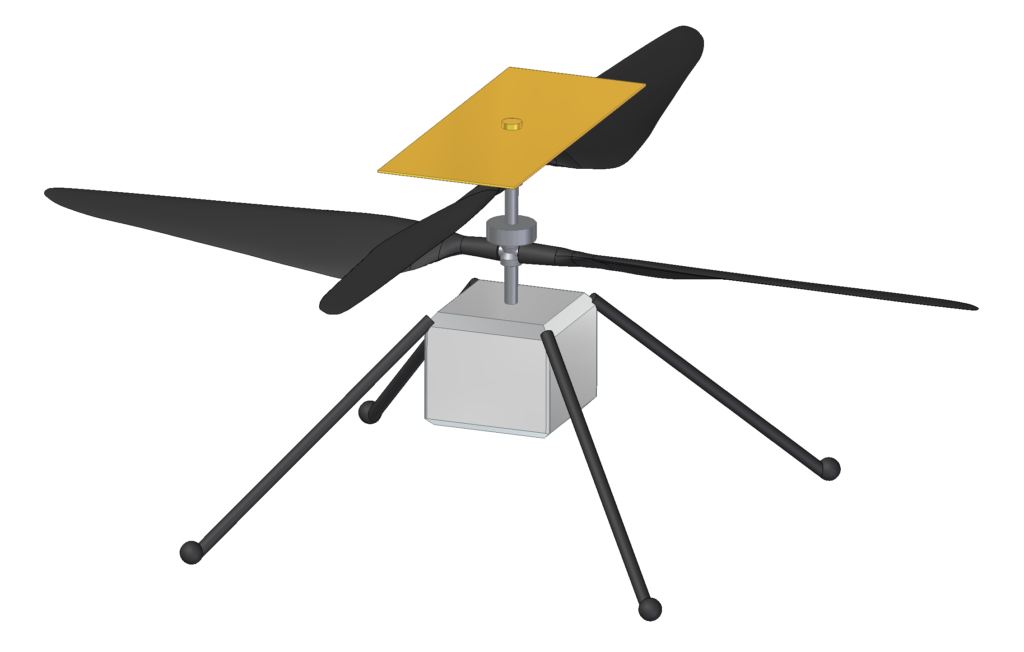
\includegraphics[width=0.7\columnwidth]{figures/ingenuity_render.png}
        % \caption{3D render of the Ingenuity Mars Helicopter.}
        \label{fig:ingenuity_render}
    \end{figure}
    Coaxial rotor system, comprising two horizontally-overlapping counter-rotating blades to mitigate reaction torque effects.
\end{column}
\begin{column}{0.6\textwidth}
    \begin{table}[H]
        \centering
        \resizebox{0.6\columnwidth}{!}{%
        \begin{tabular}{|c|c|c|}
            \hline
            \textbf{Parameter} & \textbf{Symbol} & \textbf{Value} \\
            \hline
            \hline
            Mass & $m$ & \SI{1.8}{\kilogram} \\
            \hline
            Rotor diameter & $2\,r$ & \SI{1.2}{\meter} \\
            \hline
            Blade chord & $c$ & \SI{0.24}{\meter} \\
            \hline
            \begin{tabular}{@{}c@{}}COM - upper\\rotor distance\end{tabular} & $d_{cm, u}$ & \SI{0.10}{\meter} \\
            \hline
            \begin{tabular}{@{}c@{}}COM - lower\\rotor distance\end{tabular} & $d_{cm, l}$ & \SI{0.05}{\meter} \\
            \hline
            Inertia & $I$ & \begin{tabular}{@{}c@{}}$diag(0.210, $\\$0.288, $\\$0.278)$\,\SI{}{\kilogram\square\meter}\end{tabular} \\
            \hline
        \end{tabular}
        }
        \caption{Structural parameters of the Ingenuity model.}
        \label{tab:ingenuity_parameters}
    \end{table}
\end{column}
\end{columns}
\end{frame}



\begin{frame}{Mars environment}
Compared to PowerPoint, using \LaTeX\ is better because:
\begin{itemize}
\item It is not What-You-See-Is-What-You-Get, but
What-You-\emph{Mean}-Is-What-You-Get:\\
you write the content, the computer does the typesetting
\item Produces a \texttt{pdf}: no problems with fonts, formulas,
      program versions
\item Easier to keep consistent style, fonts, highlighting, etc.
\item Math typesetting in \TeX\ is the best:
\begin{equation*}
\mathrm{i}\,\hslash\frac{\partial}{\partial t} \Psi(\mathbf{r},t) =
-\frac{\hslash^2}{2\,m}\nabla^2\Psi(\mathbf{r},t)
+ V(\mathbf{r})\Psi(\mathbf{r},t)
\end{equation*}

\end{itemize}
\end{frame}

\begin{frame}[fragile]{Getting Started}
\framesubtitle{Selecting the SINTEF Theme}
To start working with \texttt{sintefbeamer}, start a \LaTeX\ document with the
preamble:
\begin{block}{Minimum SINTEF Beamer Document}
\verb|\documentclass{beamer}|\\
\verb|\usetheme{sintef}|\\
\verb|\begin{document}|\\
\verb|\begin{frame}{Hello, world!}|\\
\verb|\end{frame}|\\
\verb|\end{document}|\\
\end{block}
\end{frame}

\begin{frame}[fragile]{Title page}
To set a typical title page, you call some commands in the preamble:
\begin{block}{The Commands for the Title Page}
\begin{verbatim}
\title{Sample Title}
\subtitle{Sample subtitle}
\author{First Author, Second Author}
\date{\today} % Can also be (ab)used for conference name &c.
\end{verbatim}
\end{block}
You can then write out the title page with \verb|\maketitle|.

To set a \textbf{background image} use the \verb|\titlebackground| command 
before \verb|\maketitle|; its only argument is the name (or path) of a graphic 
file.

If you use the \textbf{starred version} \verb|\titlebackground*|, the image 
will be clipped to a split view on the right side of the title slide.

\end{frame}

\begin{frame}[fragile]{Writing a Simple Slide}
\framesubtitle{It's really easy!}
\begin{itemize}[<+->]
\item A typical slide has bulleted lists
\item These can be uncovered in sequence
\end{itemize}
\begin{block}{Code for a Page with an Itemised List}<+->
\begin{verbatim}
\begin{frame}{Writing a Simple Slide}
  \framesubtitle{It's really easy!}
  \begin{itemize}[<+->]
    \item A typical slide has bulleted lists
    \item These can be uncovered in sequence
  \end{itemize}\end{frame}
\end{verbatim}
\end{block}
\end{frame}